\documentclass[12pt,a4paper]{article}	%es gibt noch andere Arten of course, wie book zB, aber mit article kommst du gut hin
\usepackage[utf8]{inputenc}
\usepackage[german, english]{babel} 
\usepackage[T1]{fontenc}
\usepackage{amsmath}
\usepackage{bm}
\usepackage{mathtools}

\usepackage{amsfonts}
\usepackage{amssymb}
\usepackage{makeidx}
%\usepackage{esvect}
\usepackage{hyperref}
\usepackage{amsmath}
\usepackage{listings}
\usepackage{subfigure}		%nützlich, wenn du mehrere Bilder in eine Bildumgebung packen möchtest
\usepackage{tabularx}		%für tabellen
\usepackage{chngcntr}
\counterwithin{equation}{section}	%damit Gleichung pro section durchgezählt werden und nicht insgesamt
\counterwithin{figure}{section}		%das gleiche für Bilder
\usepackage{graphicx}
%\usepackage{stackengine}
\usepackage[left=3cm,right=3cm,top=3cm,bottom=3cm]{geometry}
\usepackage[singlespacing]{setspace}	%macht einziligen Zeilenabstand. ansonsten onehalfspacing oder doublespacing

\newcommand{\etan}{\eta_{0}}
\newcommand{\R}{\vv{R}=X\vv{e_{x}}+Y\vv{e_{y}}}
\newcommand{\phid}{\dot{\phi}}
\newcommand{\Yd}{\dot{Y}}
\newcommand{\Xd}{\dot{X}}
\newcommand{\F}{\mathcal{F}}
\newcommand{\p}{\mathcal{P}}
\newcommand{\x}{\textbf}
\newcommand{\norm}[1]{\left\lVert#1\right\rVert}
\newcommand{\abs}[1]{\left\lvert#1\right\rvert}

\begin{document}
%\setcounter{section}{2}

\setlength{\parindent}{0pt}


\thispagestyle{empty}

\begin{titlepage}
	\centering
	
\includegraphics[width=0.45\textwidth]{logo_sw.jpg}\par\vspace{1cm}
	\vspace{1cm}
%	{\scshape\Large Spezialisierung\par}
	\vspace{1.5cm}
%	{\LARGE\bfseries working title\\wedge confinement in LC systems  \par}
	{\LARGE\bfseries Assignment Sheet Nr. 3\\  \par}
	\vspace{1cm}
	
	{\large	Paul Monderkamp, Matr.Nr. 2321677\par}
	\vfill
	

	\vfill

% Bottom of the page
	{\large  monderkamp@thphy.uni-duesseldorf.de \par}
	\vspace{2cm}
	%{\large Abgabedatum: 00.04.2017 \par}
\end{titlepage}

\thispagestyle{empty} %macht dass da keine Seitennummer drauf ist.
\newpage	%beendet die Seite und macht auf der nächsten weiter

%\section*{Abstract}
%
%The aim of this specialization report is to summarize the fundamental concepts that are necessary to understand the physical properties of liquid crystal systems and their formation.\\
%The final objective for the masters thesis is to investigate the phase behaviour of those systems in confined space. As a step towards this goal, the algorithm that is used for this problem is introduced and explained. To verify its validity one section of this report is dedicated to recreation of phase behaviour predicted by previous publications on the subject of liquid crystals such as those in this report.\\
%The derivation of the algorithm that is used to generate the corresponding results uses geometrical concepts to guarantee meaningful predictions about the relative positions of the molecules that make up the systems in this thesis. \\
%Beyond that all results are generated via numerical methods. The programming languages used in this thesis are \x{C}/\x{C++} for the generation of the numerical results and \x{MatLab} for the evaluation, processing and visualization of the data. 

%The aim of this bachelors thesis is to provide an overview over the most fundamental theoretical principles which form the basis for the \x{Theory of viscotaxis of microswimmers}. Exemplary geometries of swimming particles are chosen that successively illustrate phenomena typical of the behaviour of systems under the influence of this theory.\\
%Every section which deals with the investigation of a single statement of a problem is divided into two subsections. The first section gives the equations of motion and the respective solutions, and the second one explains the solutions in a physical context and discusses the implications. \\
%All results are purely achieved by analytical methods presented in the respective sections. 

%\newpage


\tableofcontents %macht ein Inhaltsverzeichnis #magic.
\thispagestyle{empty}
\newpage


\section{Exercise 1}
\subsection{Exercise 1 (a)}

\begin{figure}[h!]		
\centering
{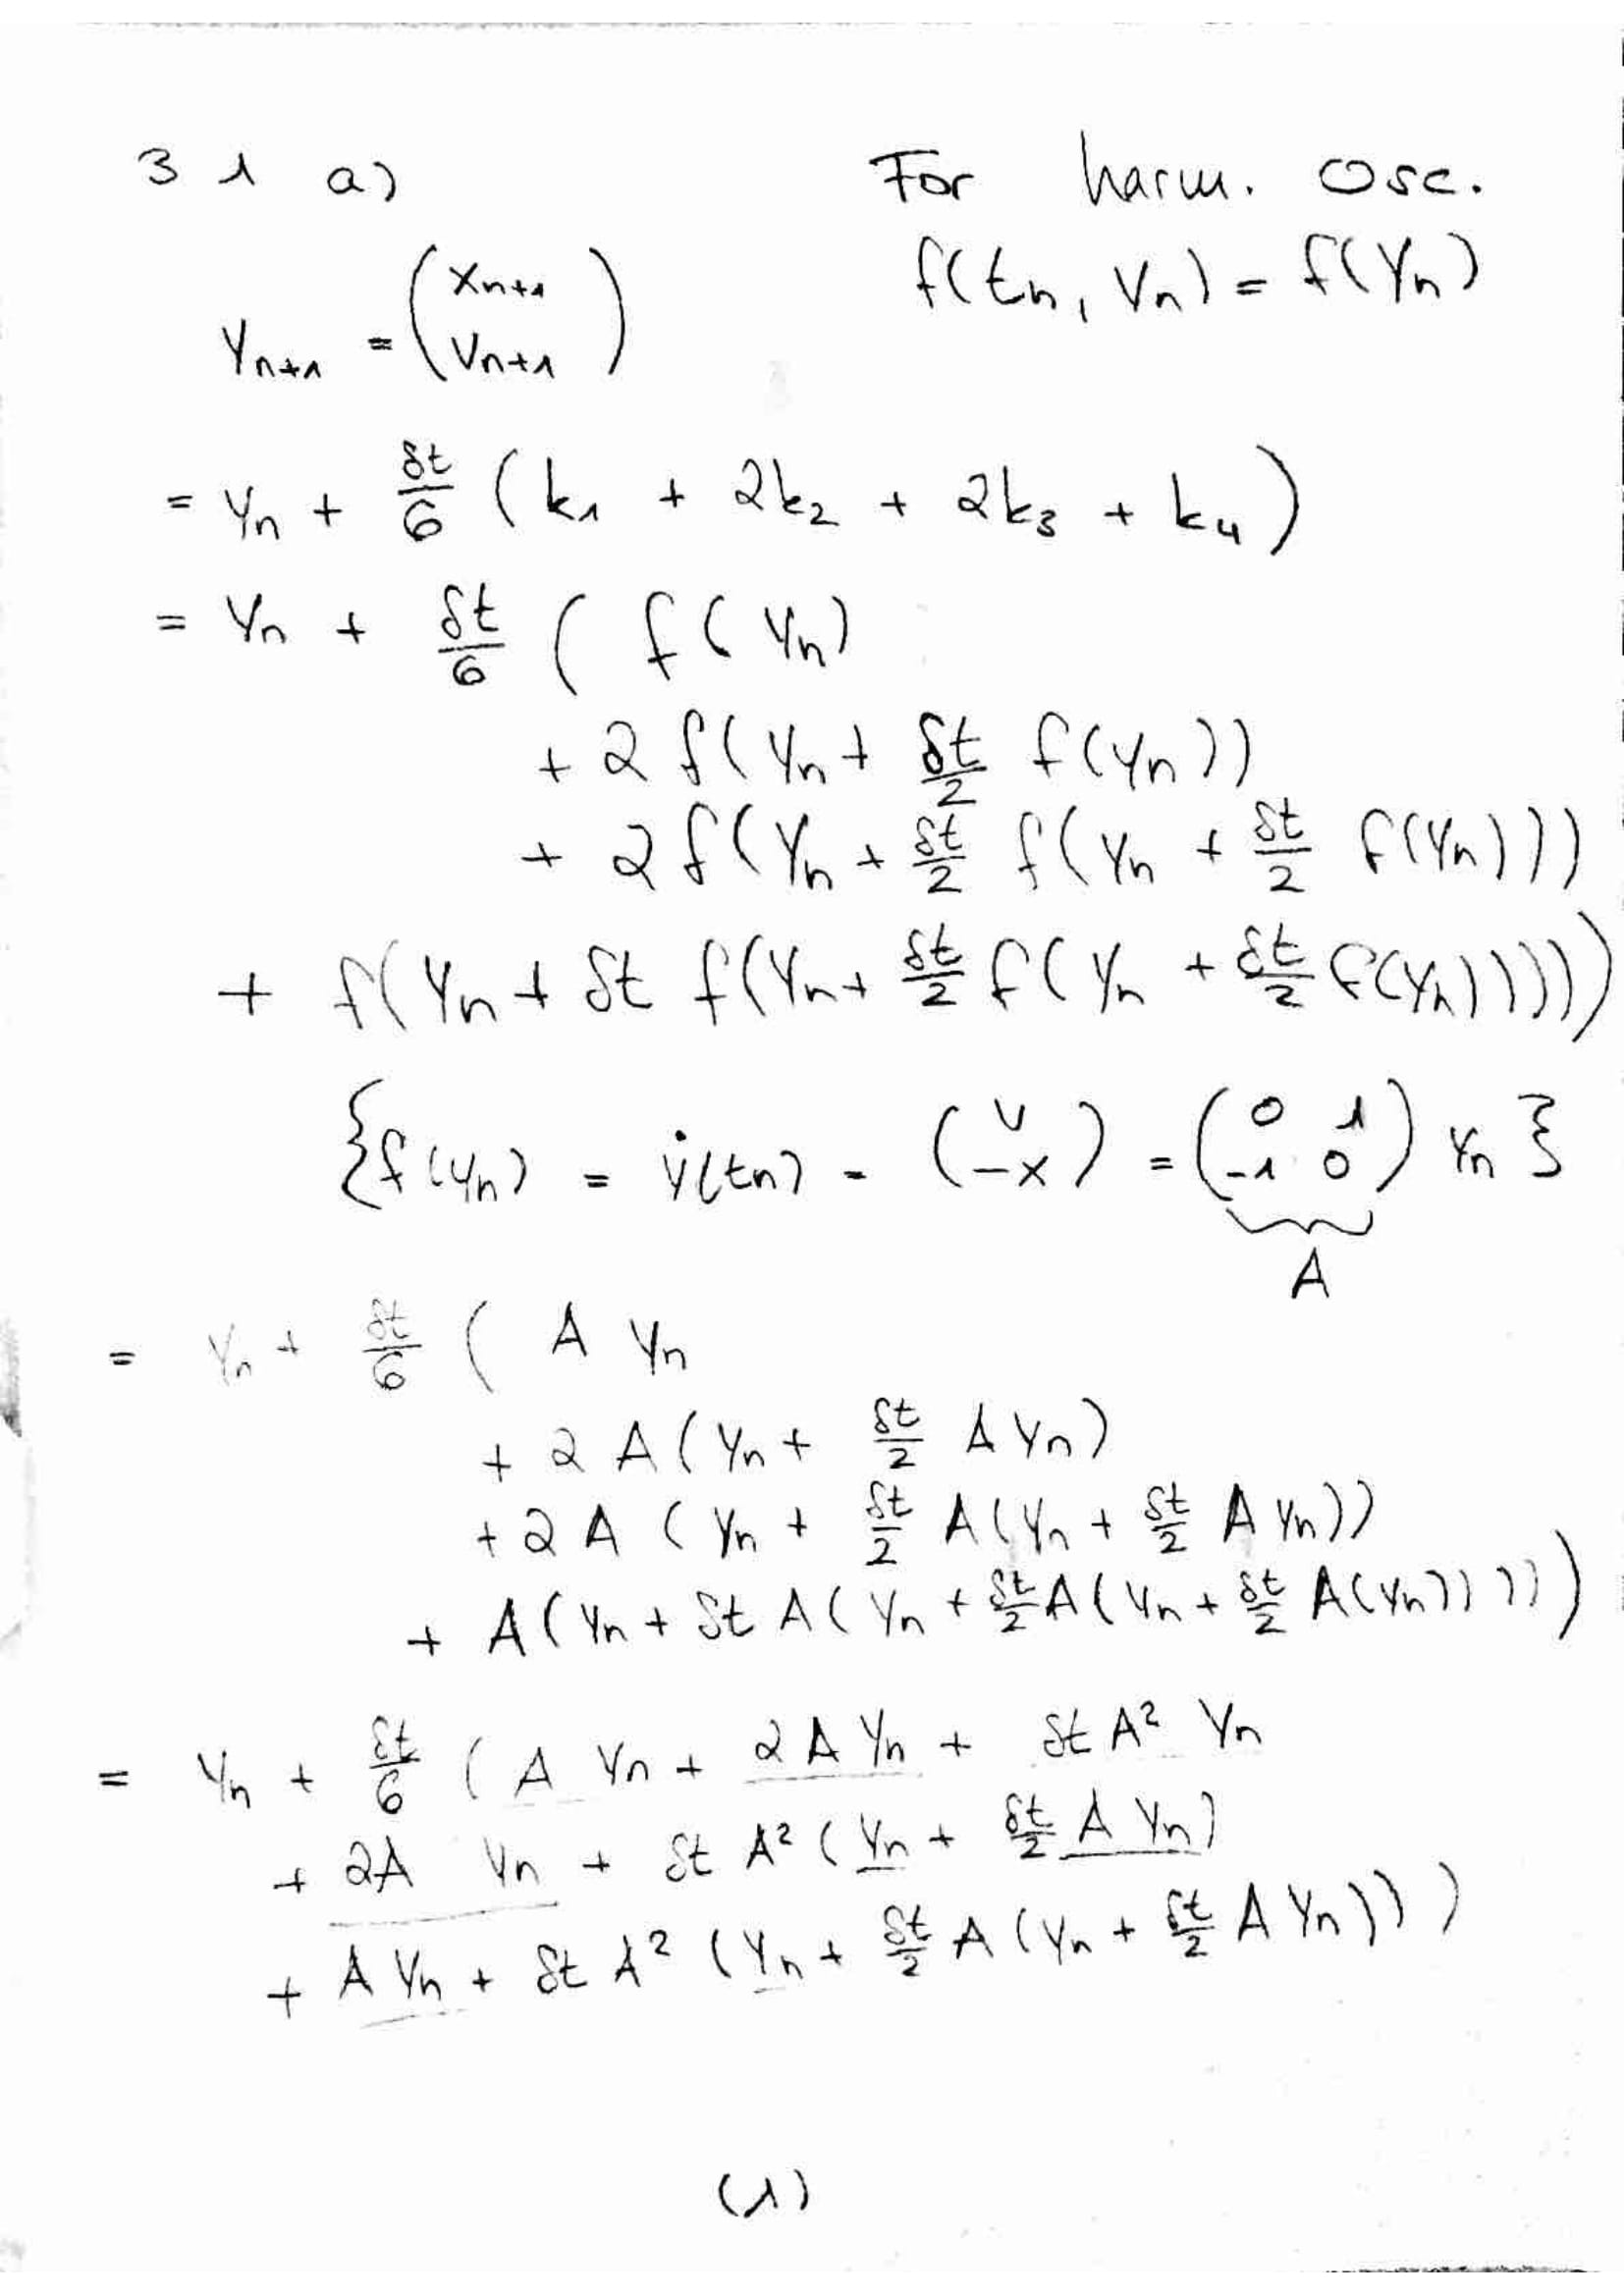
\includegraphics[width=0.9\textwidth]{3_1_a1.jpg}}		
\caption{first part of the derivation of the formula}
\end{figure}

\newpage

\begin{figure}[h!]		
\centering
{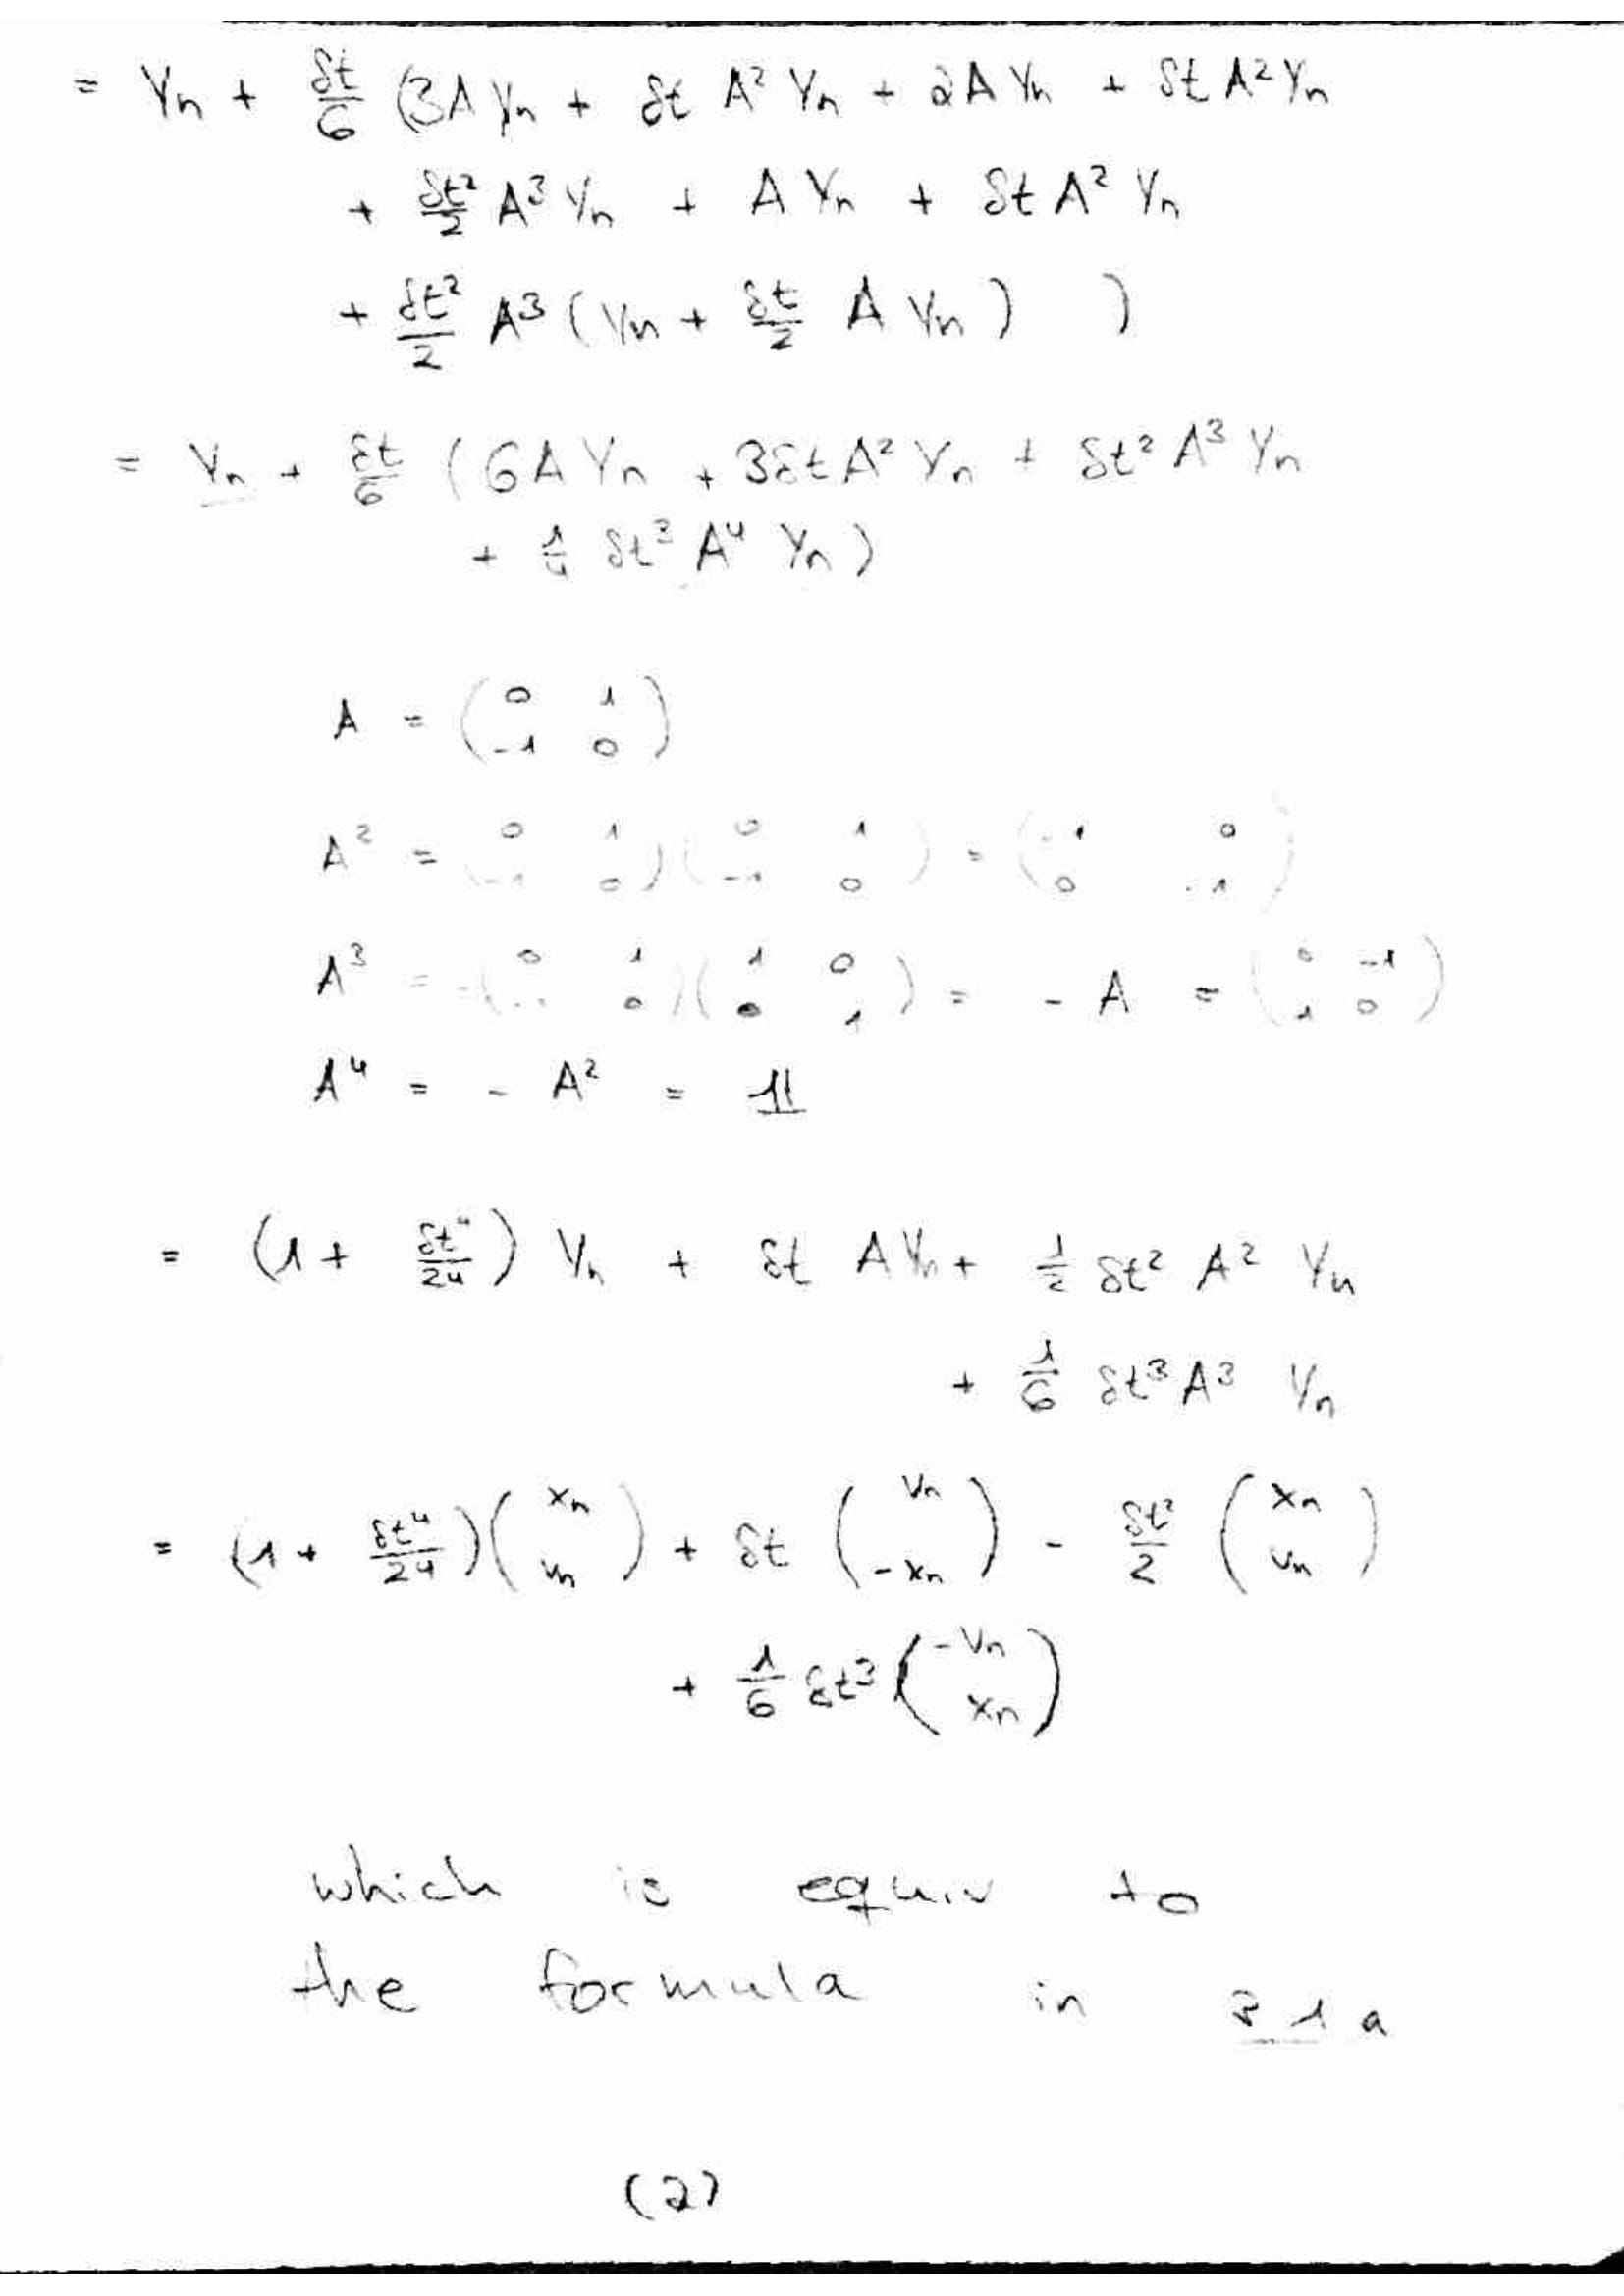
\includegraphics[width=0.9\textwidth]{3_1_a2.jpg}}		
\caption{second part of the derivation of the formula}
\end{figure}

\newpage



\subsection{Exercise 1 (b)}
\subsubsection{Code}
\lstinputlisting[language=c++]{3_1_b_main.cpp}
%\lstinputlisting{3_1_b_main.cpp}
\newpage

\subsubsection{Results}
The following results are achived via the code in the previous subsection. 
\begin{figure}[h!]		
\centering
{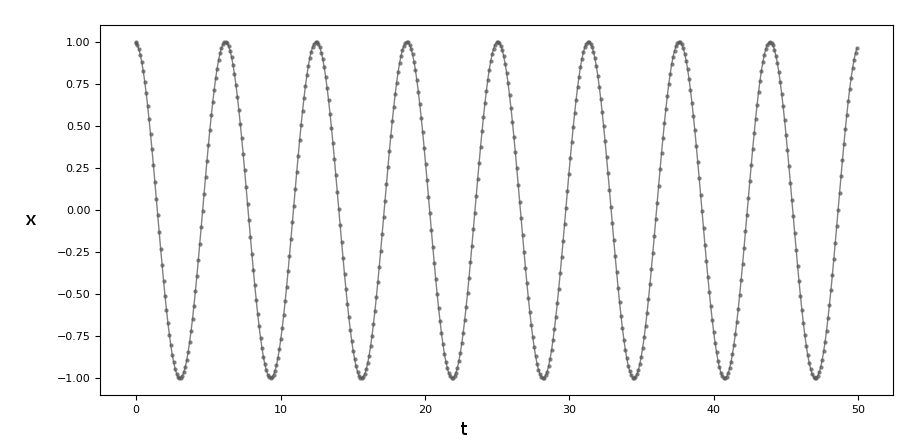
\includegraphics[width=1.0\textwidth]{1bx.png}}		
\caption{time evolution of the x coordinate of the harmonic oscillator}
\end{figure}

Figure 3.3 shows the time evolution of the x coordinate of a one dimensional harmonic oscillator solved with the Runge-Kutta 4 scheme. There is no apparent divergence from the analytical solution visible in the timeframe of the simulation.



\begin{figure}[h!]		
\centering
{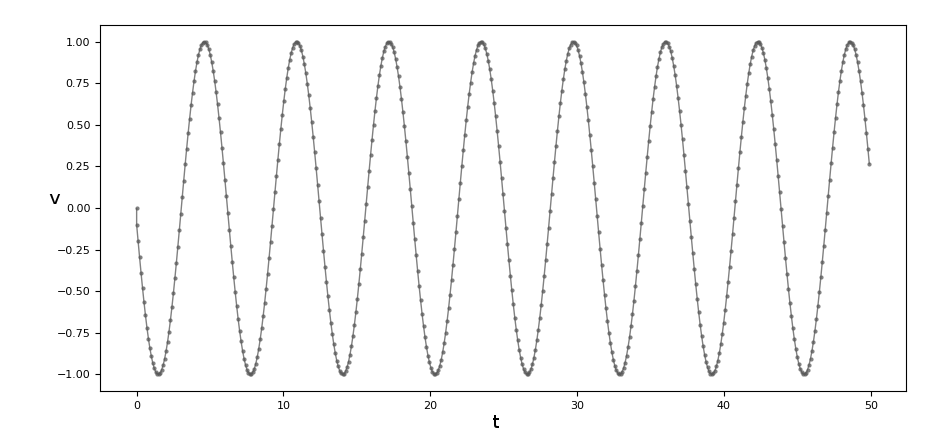
\includegraphics[width=1.0\textwidth]{1bv.png}}		
\caption{time evolution of the velocity of the harmonic oscillator}
\end{figure}

Figure 3.4 shows the time evolution of the velocity of a one dimensional harmonic oscillator solved with the Runge-Kutta 4 scheme. Similarly to the x coordinate, there is no visible instability in the timeframe of the simulation period. 

\newpage

\begin{figure}[h!]		
\centering
{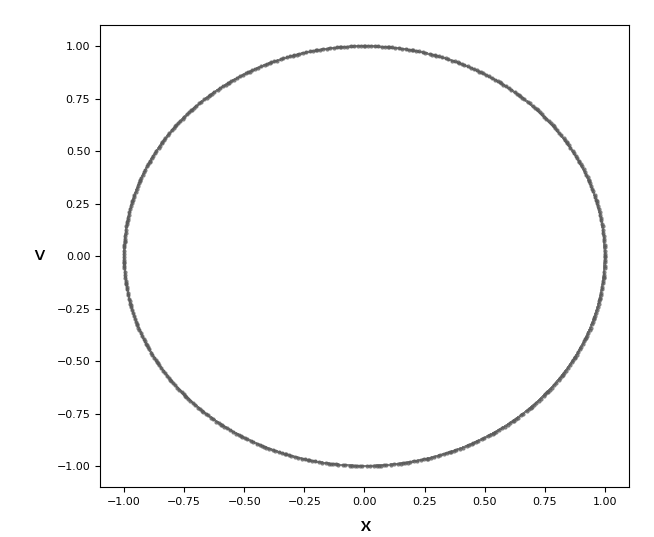
\includegraphics[width=0.5\textwidth]{1bphasespace.png}}		
\caption{phase space trajectory of the harmonic oscillator}
\end{figure}

Figure 3.5 shows the phase space profile for the simulation results above. The trajectory seems reasonably spherical. 

\section{Exercise 2}


%\begin{equation}
%\begin{pmatrix}
% 0.00227\\
%-0.00690\\
%-0.99997
%\end{pmatrix},
%\begin{pmatrix}
% 0.94354\\
% 0.33127\\
%-0.00015
%\end{pmatrix},
%\begin{pmatrix}
% -0.33126\\
%0.94351\\
%-0.00726
%\end{pmatrix}
%\end{equation}


%\section{Summary/Prospects}

%different angles wedge confinement
%\newpage


%
%\begin{equation}
%\vec{r_{1,2}}=\vec{R}\mp r\begin{pmatrix}
%\cos\phi\\
%\sin\phi
%\end{pmatrix}.
%\end{equation}


 




%\addtocontents{toc}{\protect\newpage}





%\section{Summary/ Prospects}
%
%
%\newpage



%\section{Appendix}


%\section{References}
%%\begin{enumerate}
%
%%\item i suppose it would be reasonable to give a justification for the low reynolds number and attach a source. 
%
%%%\item das hier ist ne
%%\item durchnummerierte Aufzählung.
%%\item bietet sich natürlich für die Quellen an.
%%\end{enumerate}
%%Wenn du da noch eckige Klammern drum haben willst:\\
%\renewcommand{\labelenumi}{[\theenumi]}
%\begin{enumerate}
%
%\item item 1
%URL: \\
%\url{url1} \\
%published as: item1, last visited: date


%\end{enumerate}


\newpage

%\section{Statutory Declaration}
%
%I declare that I have developed and written the enclosed thesis completely by
%myself, and have not used sources or means without declaration in the text. Any
%thoughts from others or literal quotations are clearly marked. The thesis was
%not used in the same or in a similar version to achieve an academic grading or is being
%published elsewhere.
%\\
%\\
%\\
%\\
%\underline{\hspace{7cm}}\\
%Date, Paul Monderkamp

\end{document}
